% File: 20220808005-YahyaEfeKurucay.tex
% Compile with: pdflatex -shell-escape 20220808005-YahyaEfeKurucay.tex

\documentclass{beamer}

% ---------- BEAMER THEME & COLORS ----------
\usetheme{Madrid}
\setbeamertemplate{navigation symbols}{}


% ---------- TITLE DATA ----------
\title[Kruskal's Algorithm]{Kruskal's Algorithm\\[4pt]\Large\textbf{Minimum Spanning Trees \& Union-Find}}
\author{Yahya Efe Kuruçay 20220808005}
\date{May 17, 2025} % Veya \date{\today}

% ---------- PACKAGES ----------
\usepackage{tikz}
\usetikzlibrary{arrows.meta, positioning, shapes.geometric, calc}
\usepackage{minted}
\usepackage{amsmath, amssymb}

\usepackage{ragged2e}
\usepackage{xcolor}
\definecolor{myblue}{RGB}{30, 90, 200}

% ---------- MINTED SETTINGS ----------
\setminted{
    fontsize=\scriptsize, % Kısaltılmış kod için \scriptsize yeterli olmalı
    linenos,
    bgcolor=gray!10,
    breaklines=true, % breaklines=true olarak değiştirildi, uzun satırlar için daha iyi
    autogobble,
    frame=lines,
    framesep=2mm,
    baselinestretch=0.95
}

% ---------- TIKZ STYLES ----------
\tikzset{
    vertex/.style = {circle, draw, fill=myblue!10, text=myblue, minimum size=1.5em, inner sep=1pt, font=\small\bfseries},
    edge/.style = {thick, myblue!70},
    weight/.style = {font=\scriptsize, midway, sloped, fill=white, inner sep=1pt},
    selected/.style = {edge, red, line width=1.5pt},
    rejected/.style = {edge, gray, dashed, line width=1pt}
}

% ---------- DOCUMENT ----------
\begin{document}

% Title slide
\begin{frame}
  \titlepage
\end{frame}

% Motivation
\begin{frame}{Why Minimum Spanning Trees?}
  \begin{itemize}
    \item Connect all nodes with \textbf{minimum total edge weight}.
    \item Applications:
      \begin{itemize}
        \item Network design (telecom, electrical grids)
        \item Cluster analysis
        \item Approximation for NP-hard problems (e.g., TSP)
      \end{itemize}
  \end{itemize}
\end{frame}

% Algorithm Idea
\begin{frame}{Kruskal's Approach}
\begin{enumerate}
  \item Sort edges by weight in ascending order.
  \item Add edges one by one, \textbf{skipping cycles}.
  \item Use \textcolor{red}{Union-Find} data structure for efficient cycle detection.
\end{enumerate}
\vfill
\[
\text{Time Complexity: } \mathcal{O}(E \log E)
\]
\end{frame}

% Example Graph
\begin{frame}{Step-by-Step Example: Initial Graph}
\centering
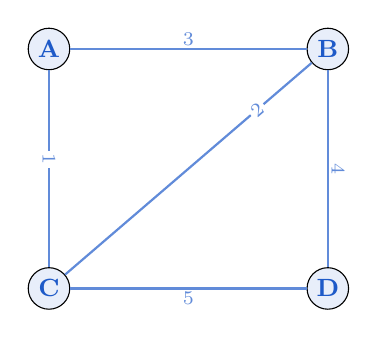
\begin{tikzpicture}[node distance=2.5cm and 3cm]
  \node[vertex] (A) {A};
  \node[vertex, right=of A] (B) {B};
  \node[vertex, below=of A] (C) {C};
  \node[vertex, right=of C] (D) {D};

  \draw[edge] (A) -- node[weight, above] {3} (B);
  \draw[edge] (A) -- node[weight, left] {1} (C);
  \draw[edge] (B) -- node[weight, right, near start] {2} (C);
  \draw[edge] (B) -- node[weight, above] {4} (D);
  \draw[edge] (C) -- node[weight, below] {5} (D);
\end{tikzpicture}
\vspace{0.5cm}
\RaggedRight
\scriptsize
\textbf{Sorted edges by weight:} \\ (A-C: 1), (B-C: 2), (A-B: 3), (B-D: 4), (C-D: 5)
\end{frame}

% Execution Steps
\begin{frame}{Edge Selection Process}
\centering
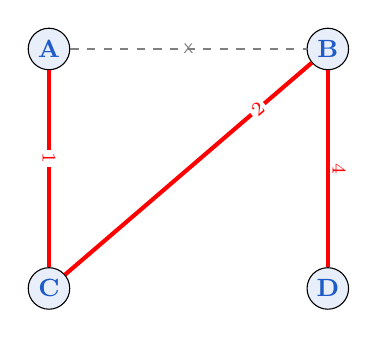
\begin{tikzpicture}[node distance=2.5cm and 3cm]
  \node[vertex] (A) {A};
  \node[vertex, right=of A] (B) {B};
  \node[vertex, below=of A] (C) {C};
  \node[vertex, right=of C] (D) {D};

  \draw[selected] (A) -- node[weight, left] {1} (C);
  \draw[selected] (B) -- node[weight, right, near start] {2} (C);
  \draw[rejected] (A) -- (B);
  \node at ($(A)!0.5!(B)$) [font=\tiny\sffamily, text=gray] {X};
  \draw[selected] (B) -- node[weight, above] {4} (D);
\end{tikzpicture}
\vspace{0.5cm}
\scriptsize
\textbf{MST Edges:} (A-C), (B-C), (B-D) \\
\textbf{Total weight:} 1 + 2 + 4 = 7
\end{frame}

% Code Implementation - Part 1: Union-Find (Kısaltılmış)
\begin{frame}[fragile]{Python Implementation: Union-Find (Core Logic)}
\begin{minted}[fontsize=\scriptsize]{python}
class UnionFind:
    def __init__(self, size):
        self.parent = list(range(size))
        self.rank = [0] * size # For union by rank

    def find(self, i): # Path Compression
        if self.parent[i] == i: return i
        self.parent[i] = self.find(self.parent[i]) # Crucial line
        return self.parent[i]

    def union(self, i, j): # Union by Rank
        root_i = self.find(i)
        root_j = self.find(j)
        if root_i != root_j:
            # Attach smaller rank tree under root of higher rank tree
            if self.rank[root_i] < self.rank[root_j]: self.parent[root_i] = root_j
            elif self.rank[root_i] > self.rank[root_j]: self.parent[root_j] = root_i
            else:
                self.parent[root_j] = root_i; self.rank[root_i] += 1
            return True
        return False
\end{minted}
\vspace{2mm} % Minted bloğu altına küçük bir boşluk
\tiny \textit{Key aspects: Initialization, path compression in find, union by rank in union.}
\end{frame}

% Code Implementation - Part 2: Kruskal's Algorithm (Kısaltılmış)
\begin{frame}[fragile]{Python Implementation: Kruskal's Algorithm (Core Logic)}
\begin{minted}[fontsize=\scriptsize]{python}
# Assumes UnionFind class is defined (previous slide)
def kruskal_algorithm(num_nodes, edges):
    # edges: list of (weight, u, v)
    edges.sort() # 1. Sort edges by weight
    
    mst_edges = []
    uf = UnionFind(num_nodes) # Initialize UnionFind
    
    for weight, u, v in edges: # 2. Iterate through sorted edges
        if uf.union(u, v): # 3. Add edge if it doesn't form a cycle
            mst_edges.append((weight, u, v))
            # Optimization: stop if MST has (num_nodes - 1) edges
            if len(mst_edges) == num_nodes - 1: 
                break 
                
    return mst_edges

# Example (conceptual):
# mst = kruskal_algorithm(4, [(1,0,2), (2,1,2), ...])
\end{minted}
\vspace{2mm}
\tiny \textit{Core steps: Sort edges, iterate, use Union-Find to check for cycles.}
\end{frame}

% Complexity Analysis
\begin{frame}{Time Complexity Breakdown}
  \begin{itemize}
    \item Sorting edges: $\mathcal{O}(E \log E)$
    \item Union-Find operations (with path compression & union by rank):
      \begin{itemize}
        \item Initialization of Union-Find: $\mathcal{O}(V)$
        \item For $E$ edges, up to $2E$ `find` and $V-1$ `union` operations.
        \item Amortized time per operation: Nearly constant, $\mathcal{O}(\alpha(V))$, where $\alpha$ is the inverse Ackermann function.
      \end{itemize}
    \item **Total Dominant Complexity:** $\mathcal{O}(E \log E)$ (due to edge sorting).
  \end{itemize}
\end{frame}

% Applications
\begin{frame}{Real-World Applications of MSTs}
\begin{columns}[T]
\column{0.33\textwidth}
\centering
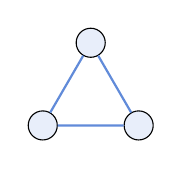
\begin{tikzpicture}[scale=0.7, transform shape]
  \node[vertex] (n1) at (0,1) {}; \node[vertex] (n2) at (-0.87,-0.5) {}; \node[vertex] (n3) at (0.87,-0.5) {};
  \draw[edge] (n1)--(n2)--(n3)--(n1);
\end{tikzpicture}
\vspace{4pt} \scriptsize Network Design

\column{0.33\textwidth}
\centering
\begin{tikzpicture}[scale=0.7, transform shape]
  \foreach \i in {1,...,3} { \node[vertex, fill=myblue!30] (c1\i) at (\i*60:0.7cm) {}; }
  \foreach \i in {1,...,3} { \node[vertex, fill=red!20] (c2\i) at (1.8cm,0) ++(\i*60-30:0.7cm) {}; }
\end{tikzpicture}
\vspace{4pt} \scriptsize Cluster Analysis

\column{0.33\textwidth}
\centering
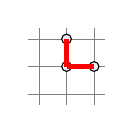
\begin{tikzpicture}[scale=0.7, transform shape]
  \draw[step=.5cm,gray,very thin] (-0.7,-0.7) grid (0.7,0.7);
  \node[vertex, minimum size=0.5em] at (0,0) {}; \node[vertex, minimum size=0.5em] at (0.5,0) {}; \node[vertex, minimum size=0.5em] at (0,0.5) {};
  \draw[selected] (0,0) -- (0.5,0); \draw[selected] (0,0) -- (0,0.5);
\end{tikzpicture}
\vspace{4pt} \scriptsize Image Segmentation
\end{columns}
\end{frame}

% Summary
\begin{frame}{Key Takeaways}
  \begin{itemize}
    \item Kruskal's is a \textbf{greedy algorithm} for finding Minimum Spanning Trees.
    \item Time complexity is primarily driven by edge sorting: $\mathcal{O}(E \log E)$.
    \item Efficiently detects cycles using the \textbf{Union-Find} data structure.
    \item Widely applicable in various network optimization and data analysis problems.
  \end{itemize}
\end{frame}

\end{document}